%\documentclass[12pt, a4j, dvipdfmx, sffamily]{jsarticle}
\documentclass[12pt, a4j, dvipdfmx, sffamily]{jsarticle}
\usepackage[dvipdfmx]{graphicx}
\usepackage[margin=9truemm, bottom=18truemm]{geometry}
\usepackage[deluxe]{otf}
\special{}

\usepackage{amsmath, physics}
\usepackage{amssymb}
\usepackage{lipsum}
\usepackage[version=4]{mhchem}


%色
\usepackage{xcolor}
\definecolor{lg}{rgb}{0.56, 0.93, 0.56} %lightgreen
\definecolor{color1}{rgb}{0.918, 0.402, 0.430}%赤
\definecolor{color3}{rgb}{0.484, 0.750, 0.316}%緑

\colorlet{thiscolor}{color3}	%テーマカラーの選択
\colorlet{linecolor}{thiscolor!150}
\colorlet{pagecolor}{thiscolor!40}
\pagecolor{pagecolor}


%ref
\usepackage[dvipdfmx, colorlinks = true, linkcolor = lg, urlcolor=blue, citecolor = lg, anchorcolor = lg]{hyperref}
\usepackage{pxjahyper, url}


%ヘッダーとフッター
\usepackage{fancyhdr}
\pagestyle{fancy}
\fancyhead{}
\fancyfoot[C]{\gtfamily\sffamily\textcolor{gray}{生物物理班\hfill\thepage}}
\renewcommand{\headrulewidth}{0pt}


%図
\usepackage{caption}
\usepackage{here}
\usepackage{wrapfig}
\captionsetup[figure]{format=plain, labelformat=simple, labelsep=period, font={sf, footnotesize}}
\renewcommand{\figurename}{Figure}
\renewcommand{\tablename}{Table}


%TikZ
\usepackage{tikz}
\usetikzlibrary{shapes.geometric}


%section関係
\usepackage{titlesec}
\titleformat{name=\section, numberless}
   [hang]
   {\vspace{2pt}\fontsize{20pt}{20pt}\selectfont}
   {\textcolor{linecolor}{■}}
   {3pt}
   {\hspace{0pt}}
   [\vspace{-5mm}\textcolor{linecolor}{\hrulefill}\vspace{-5mm}]


%tcolorbox
\usepackage{tcolorbox}
\tcbuselibrary{raster, skins}
\tcbset{	enhanced,
		colback=white,
		colframe=thiscolor!200,
		sharp corners,
		rounded corners = southeast,
		drop shadow,
		fonttitle=\gtfamily\sffamily\Large,
		fontupper=\gtfamily\sffamily,
		before upper = \parindent 1zw,
		raster column skip = 5mm,
		raster row skip = 5mm,
		raster width center=\linewidth,
		raster valign=top}

%multicol
\usepackage{multicol}
\usepackage{comment}
\setlength{\columnsep}{5mm}
\newenvironment{twocols}{\begin{multicols}{2}[\vspace{-4mm}]}{\end{multicols}}
\newenvironment{twocols*}{\begin{multicols*}{2}[\vspace{-4mm}]}{\end{multicols*}}
%%%%%%%%%%%%%%%%%%%%%%%%%%%%%%%%%%%%%%%%%%%%%%%%

\begin{document}\sffamily\gtfamily
\newpage
\section*{アロステリック制御}
\begin{tcbraster}[raster columns = 1]
	\begin{tcolorbox}[title = 生物と化学反応]
	細胞の中ではさまざまな化学反応が進行しています.
  %たとえば私たちは常に行っている呼吸に注目すると,肺に届いた酸素を全身の組織に運搬するためには,肺でできるだけ多くの酸素と結合し,それ以外の部位ではできるだけ多くの酸素を解離するような物質が必要です.
	%これをやっているのが赤血球に含まれるヘモグロビンというタンパク質です.
	%ヘモグロビンは酸素濃度がある値を超えると一気に酸素を受け取り,酸素濃度がその値を下回ると一気に酸素を手放すという性質を持っています.
  %このヘモグロビンによる酸素の結合・解離をはじめとして,生体内の化学反応の中には条件に応じて速さが変わるものが多くあります.
	その中には条件に応じて反応の進み具合が変わるものが多くあり,それによって生命活動の維持に必要な制御が行われています.
	\end{tcolorbox}
%%%
 \begin{tcolorbox}[title = 単純な化学反応 , height = 63mm]
	\begin{wrapfigure}{r}[0pt]{0.35\linewidth}
	 \centering
	 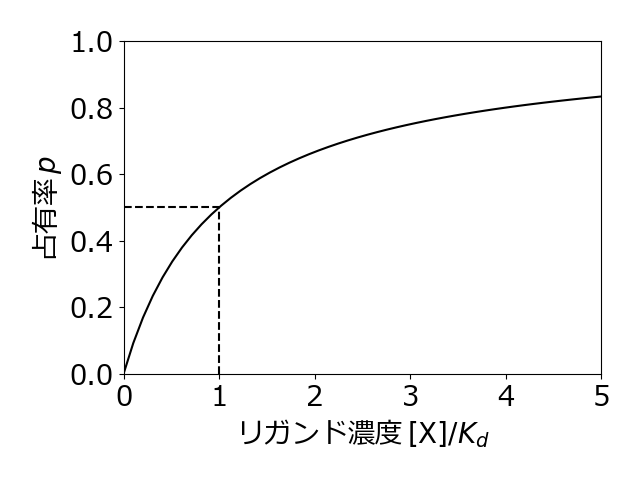
\includegraphics[width=\linewidth]{simple_poster.png}
	 \caption{単純な反応の場合の結合確率}
	\end{wrapfigure}
	たとえば,分子Yが分子Xに結合する過程を考えます.
  最も簡単な反応として
  \begin{equation*}
	 \ce{X + Y <=> XY}
  \end{equation*}
  を考えると,YはXと結合しているかしていないかの2通りの状態に分かれます.
	そこで,平衡状態でYがXと結合する確率を求めると右図のようになります.
	これより,Yは少ないXにもよく結合し,Xが多くなるにつれて結合確率が100\%に向かってゆっくりと増加していくことが分かります.	
  %この場合,各酸素濃度に対してヘモグロビンが酸素を結合する確率は右図のようになってしまい,冒頭に述べたような極端な性質が表れません.
 \end{tcolorbox}

%%%
  \begin{tcolorbox}[title = アロステリック制御 , height = 85mm]
		\begin{wrapfigure}{r}[0pt]{0.35\linewidth}
			\centering
			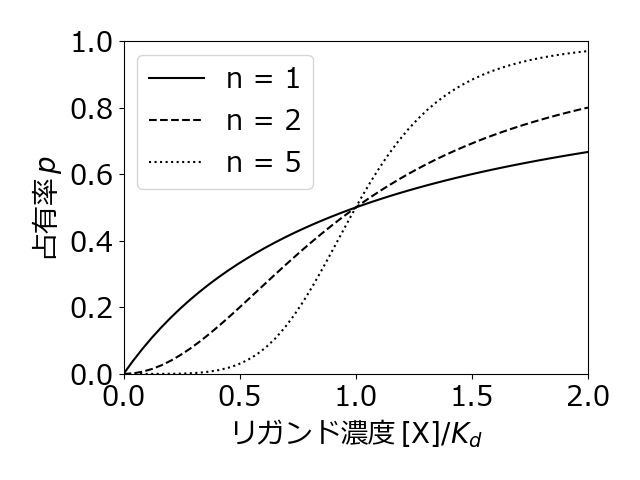
\includegraphics[width=\linewidth]{hill_poster.png}
			\caption{$n=1,2,5$の3通りについての結合部位の占有確率}
		 \end{wrapfigure}
  次に,分子Yが$n$個の結合部位を持ち,そこに分子Xが結合する過程を考えます.
	普通は結合部位一つ一つをXが埋めていくわけですが,ここでは極端な状況として,Xが一つでも結合したらYの状態が変わって,すべての結合部位をXで埋めてしまうと考えます.
	つまり
	\begin{equation*}
		\ce{$n$X + Y <=> X_{$n$}Y}
	\end{equation*}
	という反応が起こるとします.
	このとき,平衡状態においてYの$n$個の結合部位のうちXが占有する割合は右図のようになります.
	これより,$n$が増えるにつれて曲線がS字に歪み,S字の中央にあたるXの濃度を境にXの結合と解離が一気に起こるようになります.
	このS字カーブは,結合部位一つをXが埋めたときに他の結合部位に影響が出るという効果に由来します.
	これを\textbf{アロステリック効果}といい,これによる反応の制御をアロステリック制御といいます.
  \end{tcolorbox}
%%%
	\begin{tcolorbox}[title = 具体例(ヘモグロビン)]
	たとえばXとして酸素を,Yとしてヘモグロビンを考えると,$n=2$と$n=3$の間あたりのS字になることが知られています.
	これによりヘモグロビンは,酸素濃度の高い肺胞では酸素を一気に受け取り,酸素濃度の低い末梢の組織ではそれを一気に手放すという酸素の運搬を実現しています.
	\end{tcolorbox}
\end{tcbraster}
\end{document}